\begin{latin}

\section{3.34 The Minkowski function.}

The \textit{Minkowski function} of a convex set $ C $ is defined as
\begin{equation}
	M_{C}(x) = \inf\{t > 0 | t^{-1}x \in C\}.
\end{equation}
\begin{enumerate}
	\item Draw a picture giving a geometric interpretation of how to find $ M_{C}(x) $.
	\item Show that $ M_{C} $ is homogeneous, i.e., $ M_{C}(\alpha x) = \alpha M_{C}(x) $ for $ \alpha \geq 0 $.
	\item What is dom $ M_{C} $?
	\item Show that $ M_{C} $ is a convex function.
	\item Suppose $ C $ is also closed, bounded, symmetric (if $ x \in C $ then $ -x \in C $), and has nonempty interior. Show that $ M_{C} $ is a norm. What is the corresponding unit ball?
\end{enumerate}
\textcolor{red}{\textbf{Solution:}}
\\
\begin{enumerate}
	\item Finding $ t $ is easy. You only need to draw an a arrow from $ 0 $ toward $ x $. Then find the point $ (y) $ that this array exits from set $ C $. Then $ t = x/y $. As a result if this arrow does not even enters the set $ C $, we will have $ M_{C}(x) = \infty $ and  if this arrow does not exit form the the set $ C $, we will have $ M_{C}(x) = 0 $.
	\begin{figure}[H]
		\centering
		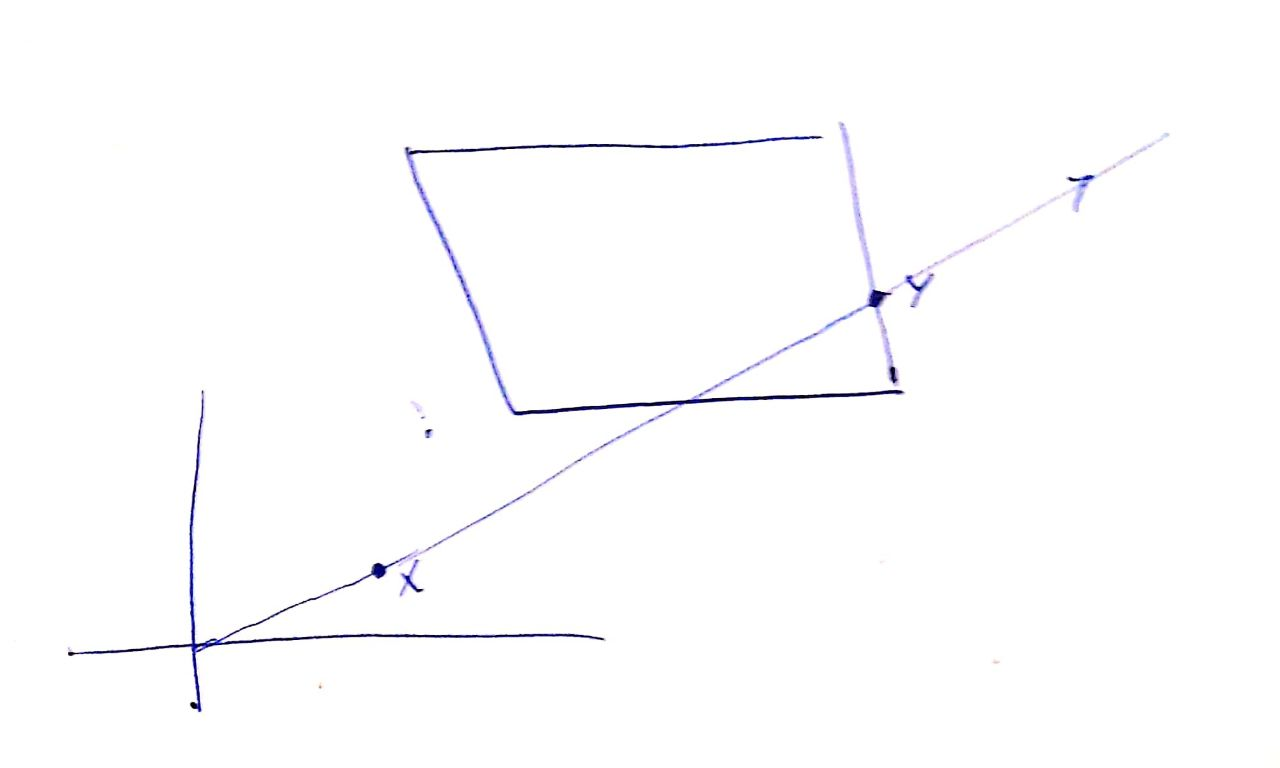
\includegraphics[width=0.45\linewidth]{Q4_Img}
	\end{figure}
	\item If $ \alpha > 0 $:
	\begin{equation*}
			M_{C}(\alpha x) = \inf \{t > 0 | t^{-1} \alpha x \in C\}
		   = \alpha \inf \{t/\alpha > 0 | t^{-1} \alpha x \in C\}
		   = \alpha M_{C}(x)
	\end{equation*}
	If $ \alpha = 0 $:
	\begin{equation*}
		M_{C}(\alpha x) = M_{C}(0) = \begin{cases}
			0 & 0 \in C \\
			\infty & 0 \notin C \\
		\end{cases}
	\end{equation*} 
	\item 
	Dom $ M_{C} = \{x | x/t \in C \text{ for some } t > 0\} $
	\item 
	Dom $ M_{C} $ is a convex set because it is  conic hull of $ C $. Suppose $ x_{1}, x_{2} \in \text{ dom } M_{C} $ so there exist $ t_{1} $ and $ t_{2} $ that $ x_{1}/t_{1} \in C $ and $ x_{2}/t_{2} \in C $. We should show that $ z = \theta x_{1} + (1 - \theta) x_{2} \in M_{C}$ for every $ 0 \leq \theta \leq 1 $.
	\\
	Because $ C $ is convex, any convex combination of $ x_{1}/t_{1} $ and $ x_{2}/t_{2} $ should be in $ C $. So 
	\begin{equation*}
		v = \frac{\theta t_{1}}{\theta t_{1} + (1-\theta) t_{2}}  (x_{1}/t_{1}) +
		\frac{(1-\theta) t_{2}}{\theta t_{1} + (1-\theta) t_{2}}  (x_{2}/t_{2}) \in C
		\Rightarrow \frac{\theta x_{1} + (1-\theta) x_{2}}{\theta t_{1} + (1-\theta) t_{2}} \in C
	\end{equation*}
	So $ M_{C}(\theta x_{1} + (1-\theta) x_{2}) \leq \theta t_{1} + (1-\theta) t_{2} $ because $ \theta t_{1} + (1-\theta) t_{2} $ was a candidate that could transfer $ \theta x_{1} + (1-\theta) x_{2} $ to $ C $ but maybe it is not the infimum value. So
	\begin{equation*}
		M_{C}(\theta x_{1} + (1-\theta) x_{2}) \leq \theta t_{1} + (1-\theta) t_{2} \leq \theta \inf \{t > 0 | x_{1}/t \in C \} + (1-\theta) \inf \{t > 0 | x_{2}/t \in C \} = \theta M_{C}(x_{1}) + (1-\theta) M_{C}(x_{2}) 
	\end{equation*}
	So it is convex.
	\item 
	For being norm, we need some homogeneity, triangle inequality, and being zero only at the origin. 
	\begin{itemize}
		\item Homogeneity: We should prove that $ M_{C}(\lambda x) = \lambda M_{C}(x) $. For $ \lambda \geq 0 $, we proved that $ M_{C}(\lambda x) = \lambda M_{C}(x) $ in part 2. By symmetry of $ C $, we also have $ M_{C}(-x) = -MC(x) $. So $ M_{C}(\lambda x) = \lambda M_{C}(x) $ for $ \lambda < 0 $ too. 
		\item Triangle inequality: 
		\begin{equation*}
			M_{C}(x + y) = 2 M_{C}(1/2x + 1/2y) \geq 2 M_{C}(1/2x) + 2 M_{C}(1/2y) = M_{C}(x) + M_{C}(y)
		\end{equation*}
		\item  Being zero only at the origin: By definition $ M_{C}(0) = 0 $. For all $ x \neq 0 $, we have $ M_{C}>0 $ because we are taking infimum on $ t > 0 $. 
	\end{itemize}
\end{enumerate}

\end{latin}